

\section{Grundlagen}
In diesem Kapitel werden die Grundlagen, die für das Grundverständnis diese Arbeit relevant sind, aufgelistet. Das Hauptaugenmerk liegt dabei auf den beiden häufigsten Steuerverfahren für ohmsche Lasten, die Phasenanschnitt- und die Schwingungspaketsteuerung. Nachteile solcher Verfahren sind verzerrte Signale, die fast nicht zu vermeiden sind. Deshalb sieht das vorliegende Konzept eine Kombination beider Steuerungsverfahren vor, wodurch eine optimale Steuerung erreicht werden soll. Daher werden nachfolgend das Aufkommen und die Auswirkungen von Oberschwingungen sowie zwischen- und subharmonischen Schwingungen erläutert. Thematisiert werden auch die Normen, die zwingend eingehalten werden müssen, denn sie setzen beiden Verfahren Grenzen.

\subsection{Auswirkung von Oberschwingungen}

Falls Oberschwingungen oder andere Netzrückwirkungen bei Betriebsmitteln auftreten, können die Geräte in ihrer Funktion beeinträchtigt oder sogar zerstört werden. Ein Beispiel dafür ist, eine Kurzzeitunterberechnung bei Schaltnetzteilen. Dabei würden sie mit extrem hohen Einschaltspitzen reagieren. Diese Spitzen könnten das 20-fache der Nennlast erreichen. Grund dafür ist, dass im einphasigen Verbrauch bei einem dreiphasigen-Wechselstromsystem der ganze Rückleitstrom über den Sternpunkt des Transformators zurückfliesst. Gibt es viele Schaltnetzteile in einem System, heben sich die Rückleiterströme nicht mehr auf, sondern sie addieren sich. Die Folge davon ist eine Sternpunktverschiebung. Ausserdem können die Oberschwingungen zum Beispiel bei Glühbirnen die Glühfadentemperatur erhöhen und somit ihre Lebensdauer verkürzen. Auch bei Dreh- oder Wechselstrommotoren und -generatoren führen Stromoberschwingungen zu zusätzlicher Erwärmung. Bei Schutzgeräten wie Distanzschutz, Überstromschutz oder Differenzialschutz können Oberschwingungen den Aufbau und die Wirkungsweise des Gerätes beeinflussen. Sind die Abstände zwischen Freileitungen und Telefonleitungen zu gering, können die Oberschwingungen die Sprachübertragung stören.



\subsection{Auftreten von verzerrten Sinusschwingungen}
Im Idealfall würde bei einer Stromversorgung überall eine perfekte sinusförmige Spannung vorliegen. Jedoch sieht dies in der Realität anders aus. Die Kurve der Spannung und des Stromes weichen massiv von einer Sinusfunktion ab. Man bezeichnet diese verzerrten Schwingungsformen im Allgemeinen als oberschwingungsbehaftetes Signal. Durch Oberschwingungsspannung können zum Beispiel Spannungsverzerrungen vorkommen, die das Überhitzen von Drehfeldmotoren verursachen. Ausserdem können bei den Oberschwingungsströmen zum Beispiel die Neutralleiter überlastet werden. Sie verursachen so einen erheblichen Schaden an einer Schaltanlage oder einer Hausinstallation.\\
Schon früh erkannte man diese Oberschwingungsverzerrungen am Netz, jedoch ist es erst heute ein ernst zu nehmendes Problem für die Versorgungsbetriebe, die Verteilnetzbetreiber und für den Endkunden, da fast jedes elektrische Gerät verzerrte Signale zurückspeist und so das Netz verunreinigt. Die grösste Herausforderung war früher die Auswirkungen von Oberschwingungsverzerrungen auf elektrische Maschinen zu erkennen. Ausserdem stellte man fest, dass Störungen in den Telefonleitungen auftraten, welche den Ton der Sprache beeinträchtigte. Allerdings kann man sagen, dass Oberschwingungsverzerrungen früher ein geringeres Gefahrenpotenzial darstellten als heute. Die heutigen Maschinen sind so konstruiert, dass sie weniger Oberwellen erzeugen. Auch bei den Verteilnetzen wird darauf geachtet, dass sie nicht mehr an der Lastobergrenze arbeiten und so ein reineres Sinussignal verwenden. Seit einigen Jahren steigt deshalb die weltweite Nachfrage nach energieeffizienten Lösungen, die nur über vermehrten Einsatz von Leistungselektronik realisierbar sind. 


\subsection{Definition der Oberschwingungen}
Die Oberschwingungen gehören in den Themenbereich \grqq\hspace{0.02cm} physische Eigenwertprobleme\grqq, folglich Wellen deren Frequenz ganzzahlige Vielfache der Grundschwingungen sind. In der Musikwelt hört man Oberschwingungsfrequenzen vor allem bei Saiteninstrumenten, wie zum Beispiel bei einer Gitarre oder einer Geige.\\
Die meisten elektrischen Geräte halten nach der perfekten Welle Ausschau. Bei Wechselstrom definiert diese Perfektion eine saubere Sinuskurve. Die daraus verwendete elektrische Spannung wechselt gleichmässig zwischen der positiven und der negativen Halbwelle hin und her. Bei einer Frequenz von \SI{50}{Hz} geschieht dies genau 50-mal pro Sekunde. Der Begriff Welle ist im Zusammenhang von Oberschwingungen jedoch nicht ganz korrekt. Eine Welle hat eine räumliche und zeitliche Ausdehnung. Die hier betrachteten Schwingungen haben aber nur eine zeitliche Ausdehnung. Die Oberschwingungsanteile in einem Wechselstromsystem sind also definiert als sinusförmige Anteile einer periodischen Schwingung, deren Frequenz einem ganzzahligen Vielfachen (Ordnungszahl) der Grundfrequenz entspricht. Die Tabelle \ref{tab:Oberschwingungfrequenz} beinhaltet die Ordnungszahlen $(n)$ in Bezug zur Frequenz $(fh)$. Es ist ersichtlich, dass zum Beispiel die 5. Oberschwingung eine Frequenz von \SI{250}{Hz} hat. Die Berechnung der Oberschwingungsfrequenz erkennt man in der Formel \ref{eq:Oberschwingungsfrequenz}.


\begin{equation}\label{eq:Oberschwingungsfrequenz}
f_h = n \cdot Grundfrequenz
\end{equation}

\begin{table}[ht!]
	
	\centering
	
	\begin{tabular}{|l|l|}
		
		\hline
		
		\begin{tabular}[c]{@{}l@{}}Ordnungszahl\\   $n$\end{tabular} & \begin{tabular}[c]{@{}l@{}}Oberschwingungs-\\frequenz (Hz)  $f_h$\end{tabular} \\ \hline
		
		1                                                            & 50                                                              \\ \hline
		
		3                                                            & 150                                                             \\ \hline
		
		5                                                            & 250                                                             \\ \hline
		
		7                                                            & 350                                                             \\ \hline
		
		11                                                           & 550                                                             \\ \hline
		
		13                                                           & 650                                                             \\ \hline
		
		…                                                            & …                                                               \\ \hline
		
		n                                                            & 50*n                                                            \\ \hline
		
	\end{tabular}
	
	\caption{Oberschwingungsfrequenzen}\label{tab:Oberschwingungfrequenz}
	
\end{table}

Die folgenden zwei Abbildungen \ref{fig:Schwing3} und \ref{fig:Schwing11} zeigen eine Grundschwingung bei 50 Hz (blau) und die jeweilige 3. und 11. Ordnung der Grundfrequenz (gelb). Mit Hilfe der verschiedenen Ordnungen können beliebige Signale dargestellt werden. In Kapitel \ref{sec:Verzerrte_Schwingung} ist dies mit einem verzerrten Signal erläutert. 

\begin{figure}[ht!]
	\begin{minipage}[t]{0.49\textwidth}
		\centering
		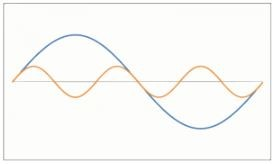
\includegraphics[scale=2]{Schwing_3.jpg}	
		\caption{Grundschwingung mit 3. Ordnung \cite{Oberwellen}}\label{fig:Schwing3}
	\end{minipage}	
	%
	\begin{minipage}[t]{0.49\textwidth}	
		\centering	
		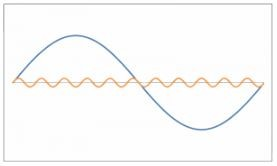
\includegraphics[scale=2]{Schwing_11.jpg}	
		\caption{Grundschwingung mit 11. Ordnung \cite{Oberwellen}}\label{fig:Schwing11}
	\end{minipage}
\end{figure}

\newpage
\subsection{Definition der zwischen- und subharmonischen Schwingungen}

Die Subharmonischen sind sinusförmige Schwingungen, deren Frequenz unterhalb der Grundfrequenz entstehen. Ein Beispiel dafür sind Schwingungen bei Frequenzen von 5, 10, oder \SI{20}{Hz} bei einer Grundfrequenz von \SI{50}{Hz}. Bei den Zwischenharmonischen handelt es sich um Sinusschwingungen, welche zwischen den harmonischen Schwingungen entstehen. Ihre Frequenz ist kein ganzzahliges Vielfaches der Grundfrequenz von \SI{50}{Hz}. Die zwei Schwingungsarten sind in der Abbildung \ref{fig:Sub und Zwischenharmonische} dargestellt. Die zwischenharmonischen Frequenzen und der damit verbundene Spannungsabfall entstehen dann, wenn elektrische Geräte eine getaktete Stromaufnahme haben deren Takt-Frequenz kein natürliches Vielfaches der Netzfrequenz ist. Ein Beispiel eines solchen Phänomens erkennt man bei direkten Umrichtern, die keinen Zwischenkreis haben. Die Folgen von zwischenharmonischen Spannungen sind Störungen auf Kommunikationseinrichtungen, die zum Beispiel Rundsteuerempfänger massiv irritieren. Die Rundsteuerempfänger hören nur auf eine bestimmte Frequenz, die kein Vielfaches von \SI{50}{Hz} ist. Sie liegen unterhalb von wenigen kHz. Fallen die Frequenzen nun genau auf die Zwischenharmonischen, so können sie vom Rundsteuerempfänger als falsche Signale interpretiert werden. Eine weitere negative Auswirkung, die Zwischenharmonische hervorrufen, sind Fehlverhalten auf die Funktion von Dimmerschaltungen. Die Thyristoren können zu früh oder zu spät zünden und so zu unfreiwilligem Lichtflackern der Beleuchtung führen. 

\begin{figure}[ht!]
	\centering
	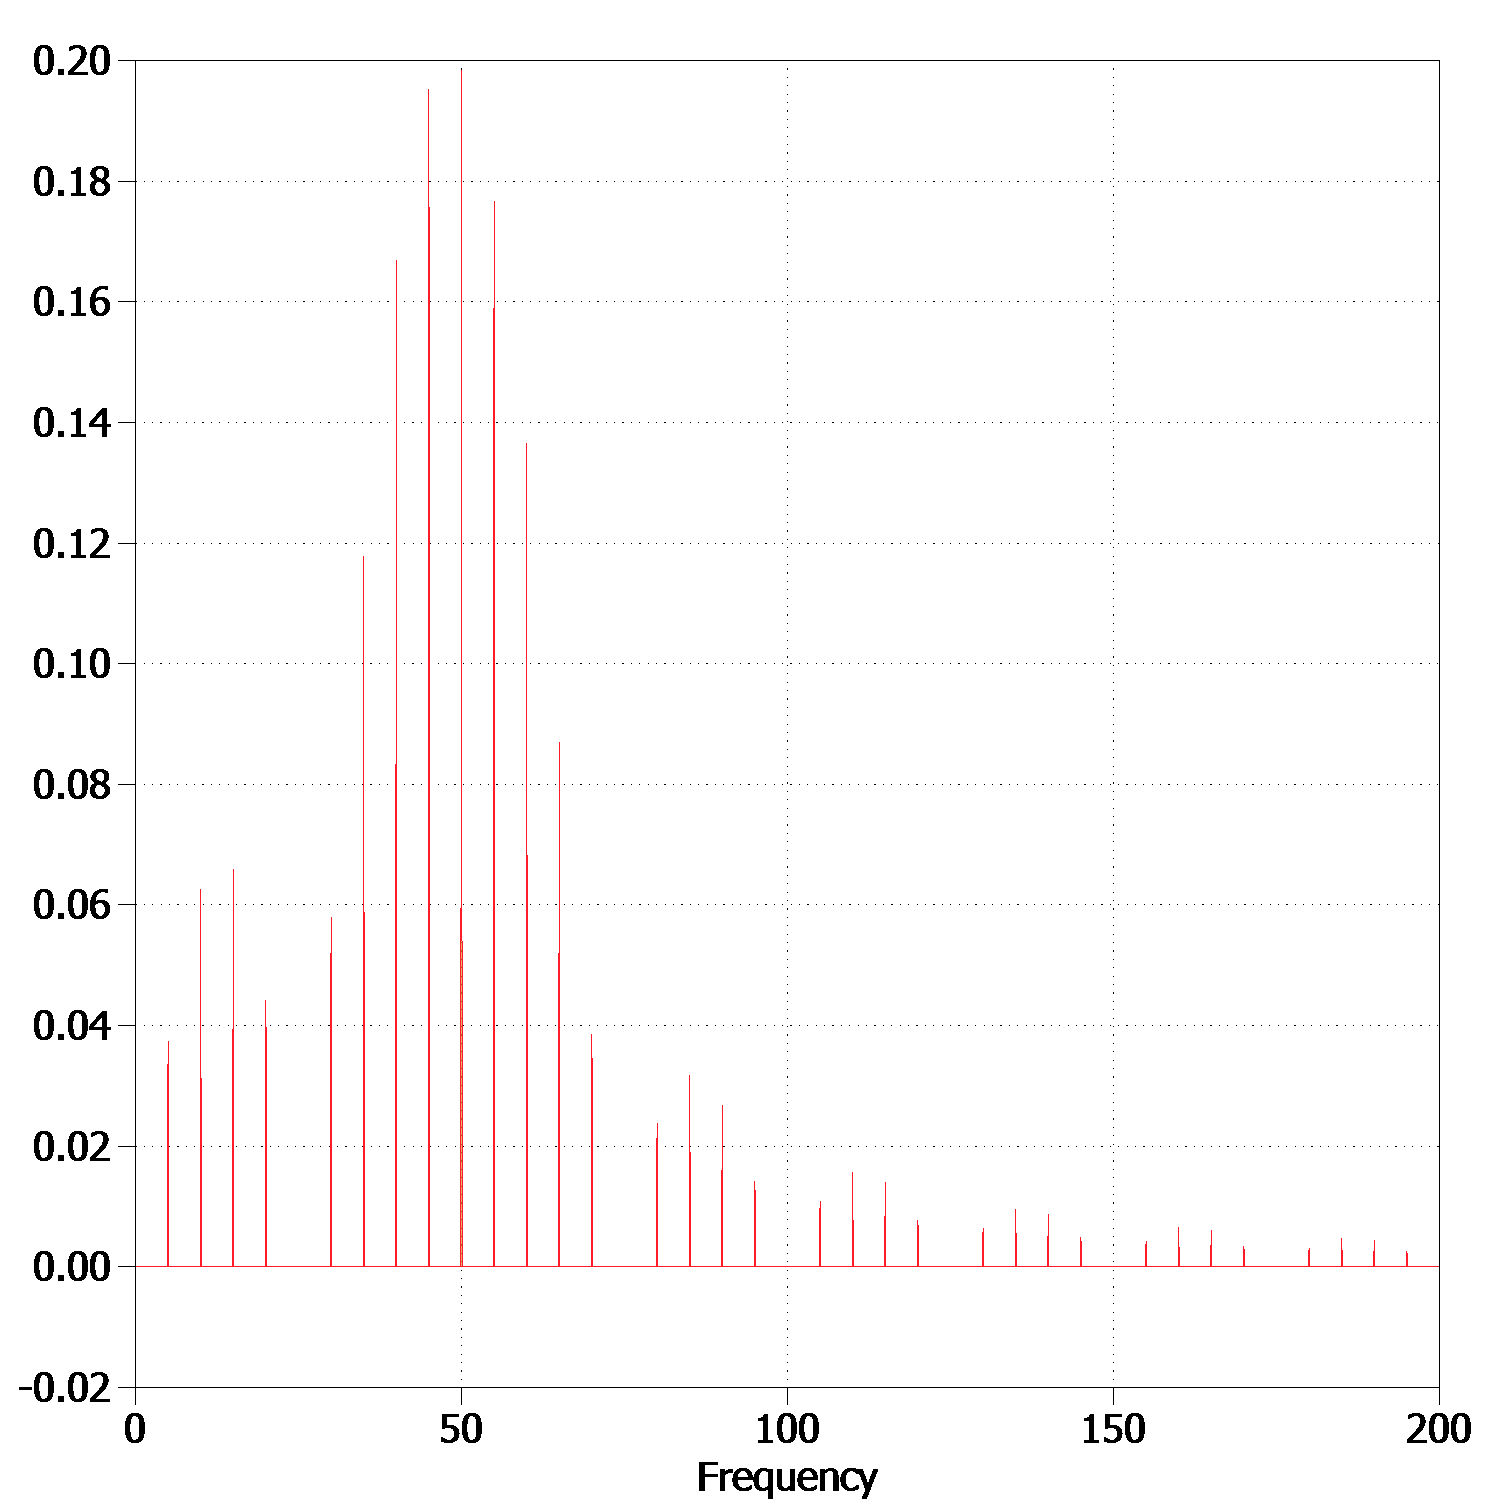
\includegraphics[scale=0.35]{sub_und_zwischenharmonische.png}	
	\caption{Sub- und Zwischenharmonische mit einer Grundfrequenz von 50 Hz}
	\label{fig:Sub und Zwischenharmonische}
\end{figure}



\subsection{Definition der verzerrten Schwingung}\label{sec:Verzerrte_Schwingung}
Eine verzerrte Schwingung entsteht durch Überlagerungen von verschiedenen sinusförmigen Wellen mit unterschiedlichen Frequenzen und Amplituden. Man kann eine solche Schwingung mit den unterschiedlichen Oberschwingungskomponenten zusammensetzen, indem man eine Sinusschwingung mit mehreren Oberschwingungen zusammenaddiert. Ein wellenförmiges verzerrtes Signal lässt sich so zu einer Grundschwingung mit mehreren harmonischen Oberschwingungen zerlegen. In Abbildung \ref{fig:Addition Oberwellen} ist diese ersichtlich, wobei die rote Kurve das verzerrte Signal darstellt. Die drei blauen Sinusschwingungen bilden die Zerlegungen zur Grundschwingung, zur 3. und 5. harmonische Oberschwingung. Addiert man die drei blauen Kurven zusammen, so erhält man wiederum das verzerrte rote Signal.

\begin{figure}[ht!]
	\centering
	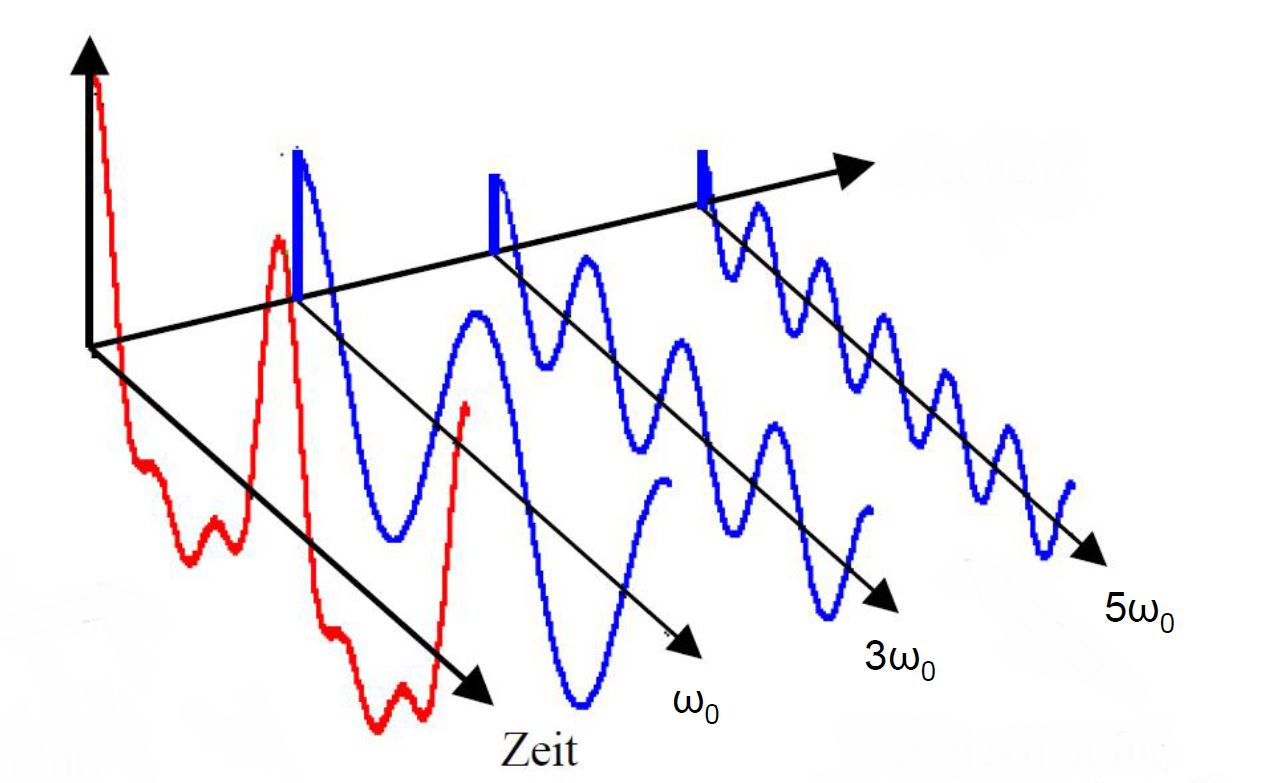
\includegraphics[scale=0.7]{verzerrtes_Signal_analysis.png}	
	\caption{Addition der verschiedenen Oberwellen \cite{analysi3}}\label{fig:Addition Oberwellen}
\end{figure}

Mit der Fourier-Transformation lassen sich die Amplitudenspektren mit den Sinuskurven bei den verschiedenen harmonischen Frequenzen übersichtlich visualisieren. Da das Amplitudenspektrum jedoch keine Informationen über die Phasenlage der einzelnen Harmonischen enthält, wird zusätzlich ein Phasenspektrum betrachtet. In der Praxis wird dieses Spektrum oft einfach weggelassen. Jedoch benötigt man für die Rekonstruktion des Eingangssignals zwingend beide Spektren. Im Kapitel \ref{sec:Simulation_mit_Matlab} konnte von Hand mit der folgenden Fourier-Reihe eine beliebige periodische Funktion als Summe von Sinus- und Cosinus-Funktionen dargestellt werden.

\begin{equation}
f(x) = {\frac{a\textsubscript{0}}{2}}+\sum_{n=1}^\infty[a\textsubscript{n} \cdot cos(nx)+b\textsubscript{n} \cdot sin(nx)]
\end{equation}


Mathematisch werden die Fourier-Koeffizienten $a\textsubscript{0}$, $a\textsubscript{n}$ und $b\textsubscript{n}$ mit den untenstehenden Formeln berechnet. Sie gelten im Frequenzbereich von 0 bis 2$\pi$: 

\begin{equation}\label{a0}
a\textsubscript{0} =  {\frac{1}{2\pi} \cdot \int_{0}^{2\pi} f(x) dx}
\end{equation}

\begin{equation}\label{an}
a\textsubscript{n} =  {\frac{1}{\pi} \cdot \int_{0}^{2\pi} f(x) \cdot cos(n \cdot \omega_0 \cdot x) dx}
\end{equation}

\begin{equation}\label{bn}
b\textsubscript{n} =  {\frac{1}{\pi} \cdot \int_{0}^{2\pi} f(x) \cdot sin(n \cdot \omega_0 \cdot x) dx}
\end{equation}

Mit den oben genannten Fourier-Koeffizienten lassen sich nun das Amplituden- und Phasenspektrum von verschiedene Signalen berechnen. Die verschiedenen harmonischen Schwingungen aber auch die Sub- und Zwischenharmonischen können so ersichtlich in einem Frequenzspektrum dargestellt werden. Mit den Formeln \ref{Amplitudenspektrum} und \ref{Phasenspektrum} berechnet man das Amplituden- und Phasenspektrum:
\begin{equation}\label{Amplitudenspektrum}
A\textsubscript{n} = {\sqrt{a\textsubscript{n}^2+b\textsubscript{n}^2}}
\end{equation}

\begin{equation}\label{Phasenspektrum}
\varphi = \arctan\left( \frac{a\textsubscript{n}}{b\textsubscript{n}}\right) 
\end{equation}



\subsection{Total Harmonic Distortion}
Oberschwingungsströme oder verzerrte Signale lassen sich bei elektrischen Geräten fast nicht vermeiden. Ein wichtiger Bezugspunkt zu den Oberschwingungsgrössen ist dabei die gesamte harmonische Verzerrung. Man nennt ihn auch den THD-Wert (Total Harmonic Distortion). Dieser Wert ist ausschlaggebend, ob ein Verbraucher an das Netz angeschlossen werden darf oder nicht. Man analysiert diesen Wert rechnerisch. Der THD-Wert gibt das Verhältnis des Effektivwertes aller Oberschwingungen zum Effektivwert der Grundschwingung an. Man verwendet ihn üblicherweise im Nieder-, Mittel-, aber auch im Hochspannungsnetz. Normalerweise wird die Verzerrung des Stromes als $THDi$ beschrieben, siehe Formel \ref{eq:THDi}, und die Verzerrung der Spannung als $THDu$, Formel \ref{eq:THDu}, angegeben. Der $THC$ (Total Harmonic Current) bezeichnet den gesamten Oberschwingungsstrom. Er wird verwendet, um den Gesamteffektivwert der Oberschwingungsströme der Ordnung 2 bis 40 zu quantifizieren, die zu einer Verzerrung der Stromkurve beitragen. Die Ordnungen sind durch die Norm so definiert, siehe Formel \ref{eq:THC}. 

\begin{equation}\label{eq:THC}
THC = {\sqrt{\sum_{n=2}^{40} I_n^2}}
\end{equation}



Die Oberschwingungsströme, welche durch Lasten in Netzwerken erzeugt werden, müssen durch die Impedanzen der Transformatoren oder Drosseln fliessen. An diesen Impedanzen kommt es zu nicht linearen Spannungsabfällen. Es werden Oberschwingungsspannungen erzeugt, die im ganzen Netz verbreitet werden. Diese können an Endgeräten eine Verzerrung der Versorgungsspannung verursachen. Somit ist die harmonische Verzerrung des Stromes $THDi$ eine direkte Ursache für die Verzerrung der Spannung $THDu$. Sie gibt das Ausmass der Verzerrung der Versorgungsspannung an. Auch dieser Wert ist definiert als Quotient des Effektivwertes der Spannungsoberschwingungsanteile bis zur 40. Oberschwingung bezogen auf den Effektivwert der Grundschwingung. 
Folgende Formel \ref{eq:THDi} berechnet die totale Verzerrung des Stromes$(THDi)$ in Prozent.
\begin{equation}\label{eq:THDi}
THDi = \frac{\sqrt{\sum_{n=2}^{40} I_n^2}}{I_{(1)}} \cdot 100 \%
\end{equation}

Parallel dazu berechnet die Formel \ref{eq:THDu} die totale Verzerrung der Spannung in Prozent:
\begin{equation}\label{eq:THDu}
THDu = \frac{\sqrt{\sum_{n=2}^{40} U_n^2}}{U_{(1)}} \cdot 100\%
\end{equation}


Je niedriger der $THDu$-Wert ist, desto besser ist die Spannungsqualität. Die Norm besagt, dass der gesamte Oberschwingungsgehalt den Wert von 8\% nicht überschreiten darf. Dazu kommt, dass heute üblicherweise für die Verzerrung die $THD$-Werte angegeben sind und nicht wie früher die Oberschwingungsgehalte (Klirrfaktore).\\







\newpage
\subsection{Phasenanschnittsteuerung}\label{sec:Phasenanschnittsteuerung}
Bei der Phasenanschnittsteuerung wird das Sinussignal über einen TRIAC geführt. Ein TRIAC besteht aus zwei antiparallel geführte Thyristoren. Die Thyristoren zünden ab einem eingestellten Zündwinkel nach jedem Nulldurchgang. Je später der TRIAC eingeschaltet wird, desto kleiner wird die mittlere Leistung über der Last. Der Zündwinkel kann von 0\textdegree \hspace{0.02cm} bis 180\textdegree \hspace{0.02cm} eingestellt werden, wobei bei 0\textdegree \hspace{0.02cm} die maximale Leistung und bei 180\textdegree \hspace{0.02cm} keine Leistung über der Last anliegt. Der Vorteil bei einer solchen Schaltung ist der sehr geringe Leistungsverlust bei der Regelung der Spannung und des Stromes. Zudem ist die Phasenanschnittsteuerung viel kompakter aufgebaut als komplizierte regelbare Schaltnetzteile, die auch einen geringen Leistungsverlust haben.
Das Problem bei der Phasenanschnittsteuerung ist, dass diese Schaltung harmonische Oberschwingungen produziert und so unerwünschte Effekte für den Netzbetreiber verursacht. Ein weiteres Problem betrifft den nicht-sinusförmigen Stromverlauf. Da Strom und Spannung nicht den gleichen Verlauf haben, tritt eine Verzerrungsblindleistung auf. Der Strom verläuft zeitlich der Spannung nach und wirkt so wie eine Induktivität. Deshalb wird dieses Verfahren von den Elektrizitätswerken nur bei kleinen Leistungen, bei symmetrischen Anschnittsteuerung von Wärmegeräten toleriert. Bei grösseren Leistungen wird deshalb die Schwingungspaketsteuerung verwendet. Auf der Abbildung \ref{fig:Phasenanschnitt1} ist ersichtlich, wie der Phasenanschnitt bei einer Netzspannung aussieht. Die grau gezeichnete Kurve ist die normale Netzspannung und die rote ist die Spannung, welcher an der Last anliegt bei einem Winkel von 135\textdegree\hspace{0.02cm}. Die Netzspannung wird somit nach \SI{7.5}{ms} eingeschaltet und nach dem Nulldurchgang wieder gelöscht. Dies wiederholt sich bei jeder Halbwelle. Man erkennt anhand der Fläche unter den Kurven, dass die Leistung der zwei Phasenanschnittswinkeln von 135\textdegree\hspace{0.02cm} und 45\textdegree\hspace{0.02cm} kleiner ist als die der Netzspannung. 

\begin{figure}[ht!]
	\centering
	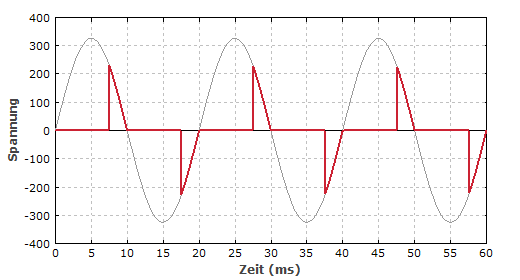
\includegraphics[scale=0.7]{phasenanschnittsteuerung1.png}	
	\caption{Phasenanschnitt mit einem Winkel von 135\textdegree \cite{Phasenanschnittsteuerung}}\label{fig:Phasenanschnitt1}
\end{figure}
\newpage
\begin{figure}[ht!]
	\centering
	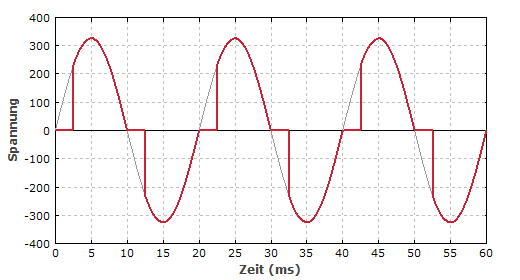
\includegraphics[scale=0.7]{phasenanschnittsteuerung2.png}	
	\caption{Phasenanschnitt mit einem Winkel von 45\textdegree \cite{Phasenanschnittsteuerung}}\label{fig:Phasenanschnitt2}
\end{figure}

In der Abbildung \ref{fig:Phasenanschnitt2} ist ersichtlich, dass die Phase früher gezündet wurde, wodurch an der Last eine grössere Leistung resultiert.



\subsection{Schwingungspaketsteuerung}\label{sec:Schwingungspaketsteuerung}
In diesem Verfahren wird nicht wie bei der Phasenanschnittsteuerung die Form der Halbwellen verändert, sondern die Zeitdauer der Halbwellen, welche an der Last anliegen. Der Vorteil dabei ist, dass nahezu keine Verschiebungsblindleistung in der Grundschwingung auftritt. Die Verluste von elektrischen Geräten können so minimiert werden. Die Paketdauer $T_0$ und die Einschaltzeit $T_E$ sind bei der Schwingungspaketsteuerung von grosser Wichtigkeit, wobei letztere verändert wird. Wenn z.B. eine Paketdauer 10 Halbwellen hat, und 5 Halbwellen eingeschaltet sind, liegt die halbe Leistung über der Last an. Anders als bei der Phasenanschnittsteuerung entstehen bei dieser Ansteuerungsart keine harmonischen Oberwellen, dafür treten aber sub- und zwischenharmonische Schwingungen auf. In Abbildung \ref{fig:Schwingungspaketsteuerung} ist ersichtlich, wie vier von den total sechs Halbwellen pro Paket eingeschaltet sind. Dies ergibt eine Leistung, welche ${2}/{3}$ so gross ist wie die der normalen Netzspannung.

\begin{figure}[ht!]
	\centering
	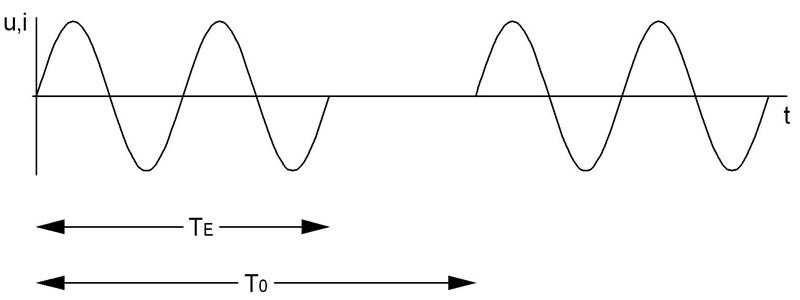
\includegraphics[scale=0.5]{Schwingungspaketsteuerung.png}	
	\caption{Schwingungspaketsteuerung ${2}/{3}$ der Leistung \cite{Schwingungspaketsteuerung}}\label{fig:Schwingungspaketsteuerung}
\end{figure}

Dabei ergibt sich aus dem Verhältnis von Einschaltdauer zu Periodendauer das Tastverhältnis.

\begin{equation}\label{eq:Einschaltverhältnis}
a = \frac{T_E}{T_0}
\end{equation}

\subsection{Leistungsfaktor}\label{sec:Leistungsfaktor}
Der Leistungsfaktor wird in der Leistungselektronik meistens dafür verwendet, um das Verhältnis des Betrages der Wirkleistung $P$ zur Scheinleistung $S$ anzuzeigen. Der Wert kann dabei zwischen 0 und 1 variieren. Wobei man sagen kann, dass je geringer der Wert ist, desto ineffizienter wird die Energie des Netzbetreibers genutzt. Um die beiden Ansteuerungsverfahren zu vergleichen, ist der Leistungsfaktor der Verfahren zu bestimmen. Bei der Phasenanschnittsteuerung geht der Leistungsfaktor bei einem kleinem Zündwinkel gegen 1, da das Verhältnis der umgesetzten Leistung als Funktion des Zündwinkels $P_{\alpha}$ zur maximalen Leistung $P_0$ auch 1 ist. Je grösser der Zündwinkel gewählt wird, desto kleiner wird $P_{\alpha}$ und entsprechend auch der Leistungsfaktor. Bei der Schwingungspaketsteuerung ist der Leistungsfaktor abhängig von dem Verhältnis der Einschaltdauer der Pakete zu den Netzperioden. Je grösser die Einschaltzeit ist, desto grösser ist der Leistungsfaktor. Die genauere Herleitung der beiden Faktoren \ref{eq:lamda_p_n} und \ref{eq:lamda_s_n} sind im Unterkapitel \ref{sec:Leistungsfaktor_Phasenanschnittsteuerung} und \ref{sec:Leistungsfaktor_Schwingugnspaketsteuerung} beschrieben. In der Abbildung \ref{fig:Leistungsfaktor} ist ersichtlich, wie sich der Leistungsfaktor bei den beiden Steuerungsarten verhält \cite{Leistungselektronik}.

\begin{figure}[ht!]
	\centering
	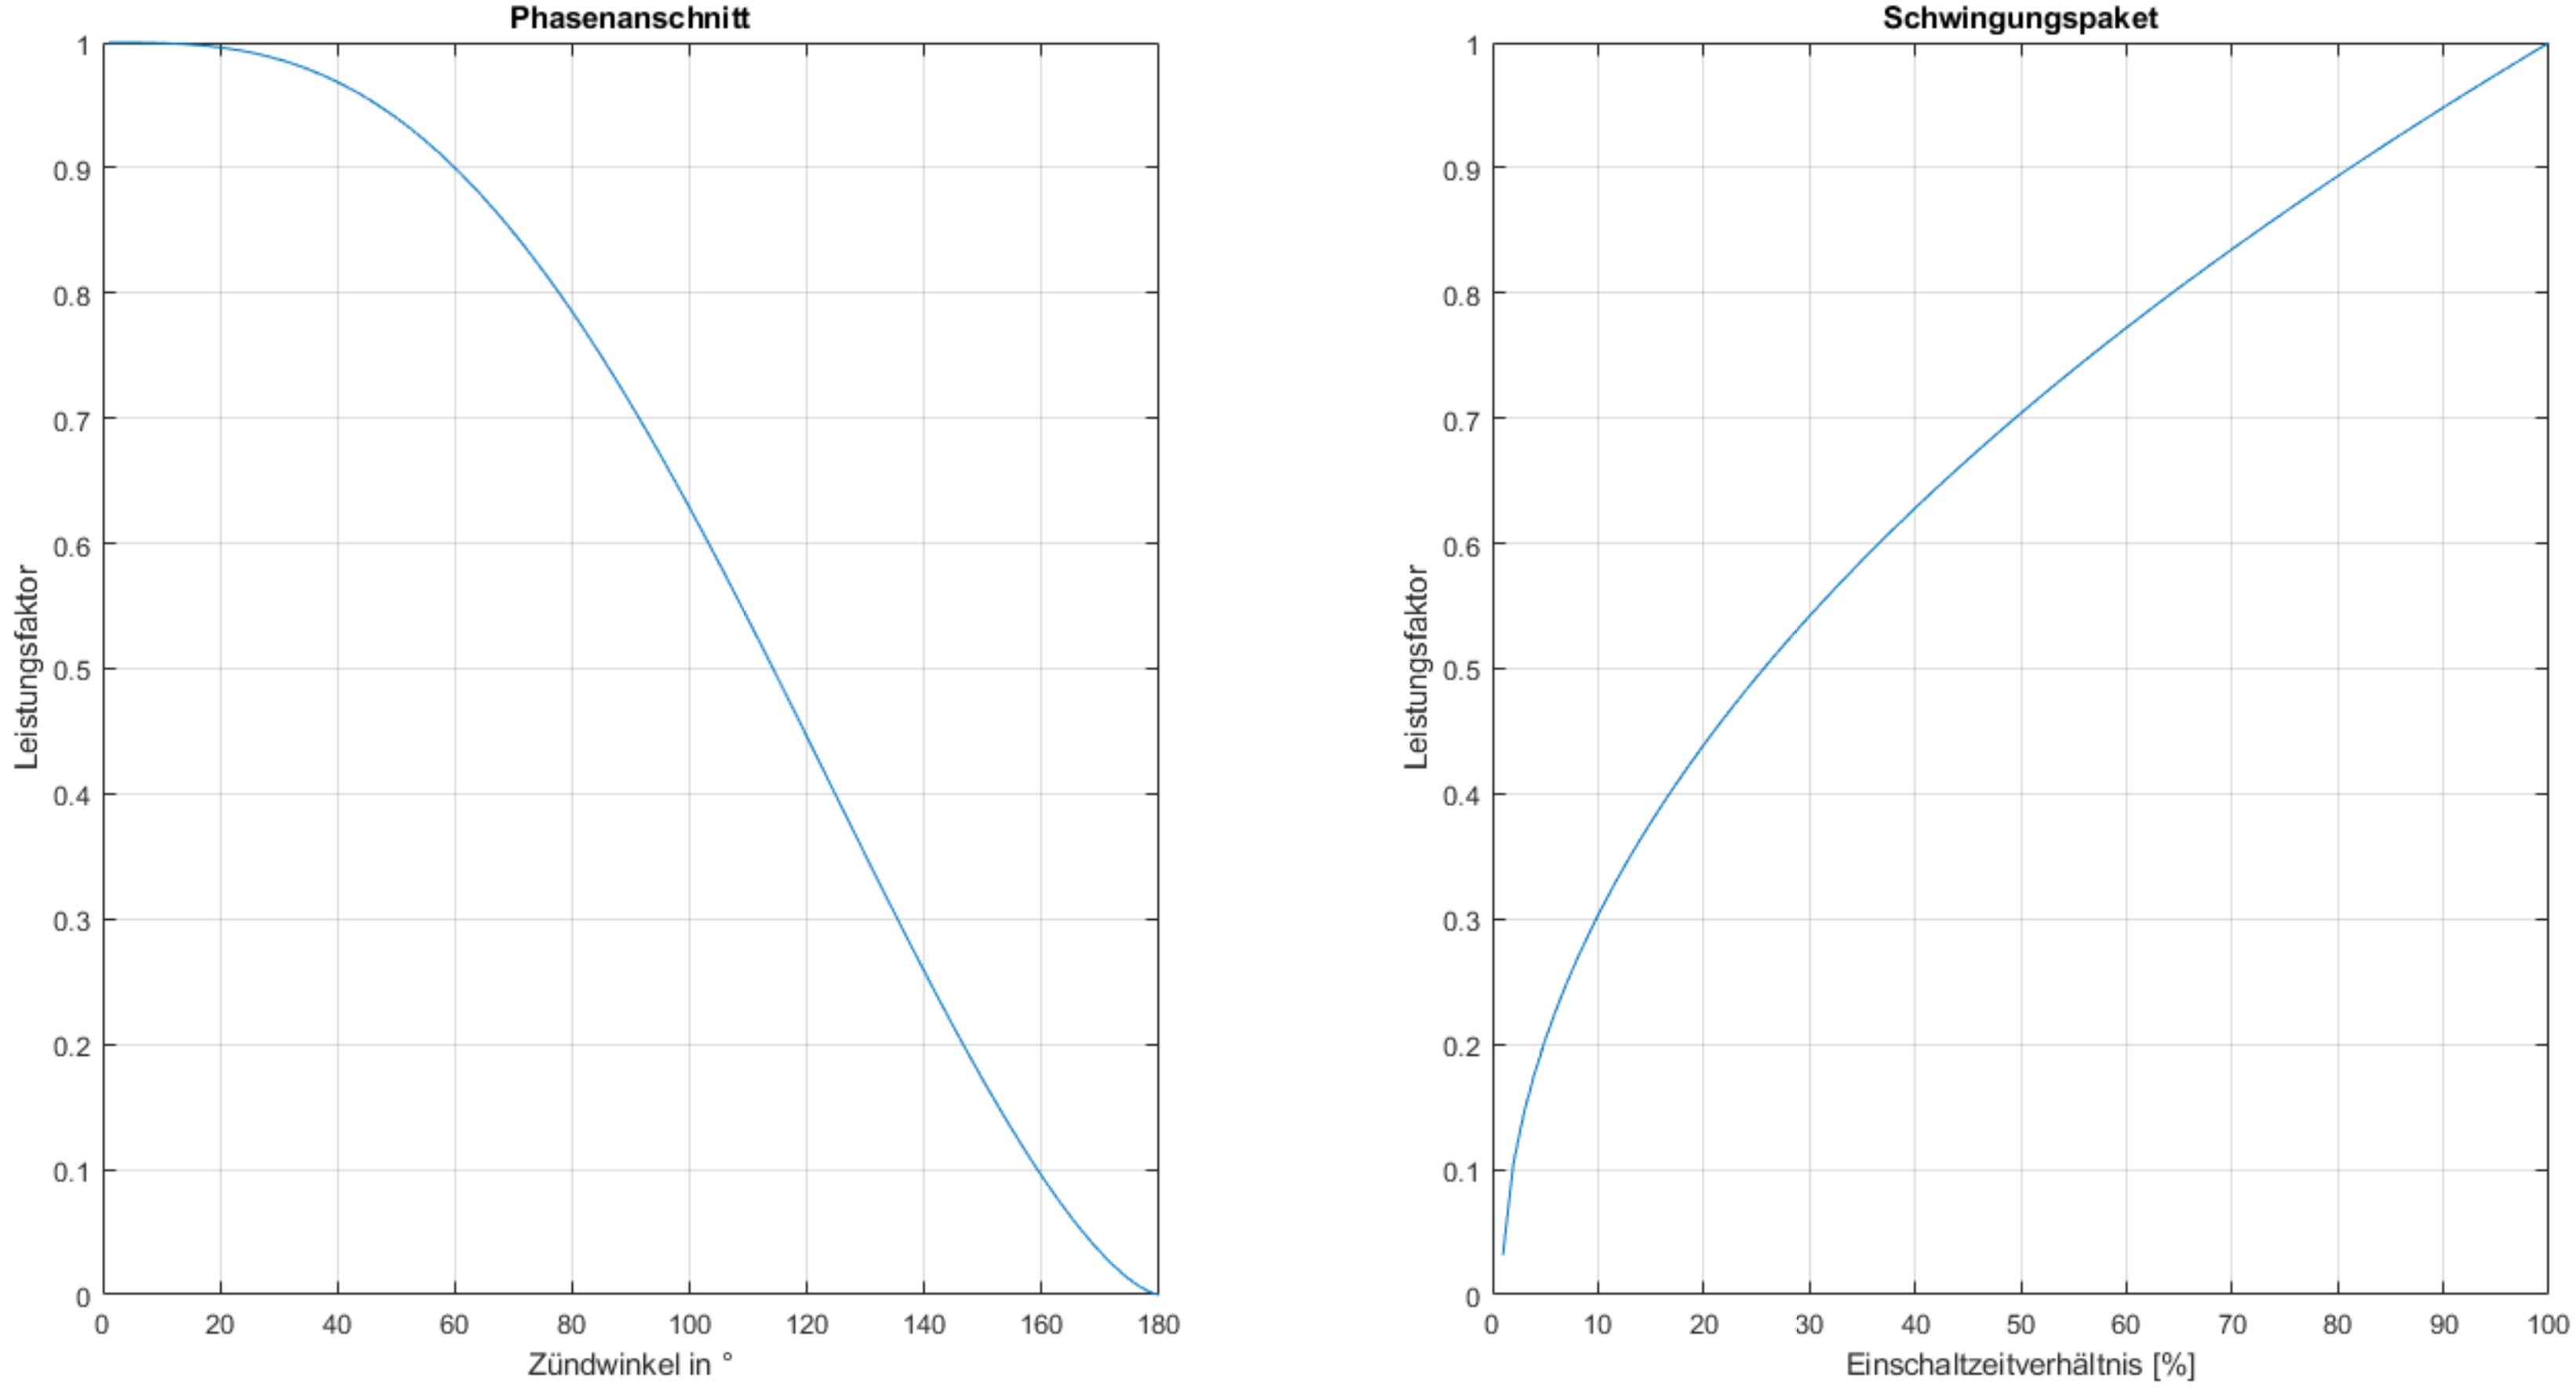
\includegraphics[width=\textwidth]{Leistungsfaktor.png}	
	\caption{Leistungsfaktor von Phasenanschnitt- und Schwingungspaketsteuerung}\label{fig:Leistungsfaktor}
\end{figure}

Der Vergleich zeigt, dass sich für beide Verfahren bei gleicher Reduzierung der gebrauchten Leistung gegenüber der maximalen möglichen auch die gleichen Leistungsfaktoren ergeben. Bei der Schwingungspaketsteuerung wird die verzerrte Leistung hauptsächlich durch die subharmonischen Schwingungen verursacht, wobei bei der Anschnittsteuerung die harmonischen die Ursachen für die Verzerrleistung sind. Dies bedeutet, dass beide Verfahren einen gewissen Einfluss auf die Stabilität des Stromnetzes, die sogenannte Netzrückwirkung, haben.
\newpage
\subsubsection{Leistungsfaktor Phasenanschnittsteuerung}\label{sec:Leistungsfaktor_Phasenanschnittsteuerung}
Der Leistungsfaktor ist definiert als Verhältnis von Wirkleistung zu Scheinleistung \cite{Leistungselektronik}. 
\begin{equation}\label{eq:lamda_p}
\lambda = \frac{P_{\alpha}}{S}
\end{equation}

Ist der Lastkreis nur Ohmsch belastet, so kann der Leistungsfaktor wie folgt beschrieben werden:
\begin{equation}\label{eq:lamda_ohmisch belastet}
\lambda =\sqrt{\frac{P_{\alpha}}{P_{0}}} 
\end{equation}
\\
Die Schein- und Wirkleistung im Lastkreis lassen sich mit den folgenden Formeln definieren:

\begin{equation}\label{eq:Scheinleistung}
S = I_L \cdot U_{UN}   
\end{equation}

\begin{equation}\label{eq:Wirkleistung}
 P_{\alpha} = I_L^2 \cdot R_L    
\end{equation}

Der Laststrom wird mit folgender Formel beschrieben:
\begin{equation}\label{eq:Laststrom}
I_L = \sqrt{1-\frac{\alpha}{\pi}+\frac{1}{2\pi} \cdot sin(2\alpha)} \cdot \frac{U_{UN}}{R_L}
\end{equation}

Wenn der Zündwinkel $\alpha$ = 0 beträgt, wird im Lastwiderstand $R_L$ die maximale Leistung $P_0$ in Wärme umgesetzt:

\begin{equation}\label{eq:Wirkleistung_bei_maximaler_alpha=0}
P_{0} = \frac{ U_{UN}^2}{R_L}  
\end{equation}

Mit den beiden Gleichung \ref{eq:Laststrom} und \ref{eq:Wirkleistung} lässt siche folgende Formel herleiten:

\begin{equation}\label{eq:p_alpha_neu}
P_{\alpha} = \left(1-\frac{\alpha}{\pi}+\frac{1}{2\pi} \cdot sin(2\alpha)\right)  \cdot \frac{U_{UN}^2}{R_L}
\end{equation}
 

Die auf den Maximalwert bezogene Leistung folgt somit der Gleichung:
\begin{equation}\label{eq:P_alpha_P_0}
\frac{P_{\alpha}}{P_0} = 1-\frac{\alpha}{\pi}+\frac{1}{2\pi} \cdot sin(2\alpha) 
\end{equation}

Setzt man die Gleichung \ref{eq:P_alpha_P_0} in die Formel des Leistungsfaktors \ref{eq:lamda_ohmisch belastet} so erhält man folgende Formel:
\begin{equation}\label{eq:lamda_p_n}
\lambda = \sqrt{1-\frac{\alpha}{\pi}+\frac{1}{2\pi} \cdot sin(2\alpha)}
\end{equation}

Man erkennt, dass der Leistungsfaktor bei rein ohmschen Belastung nur vom Einschaltwinkel abhängig ist. Die Eingangsspannung, der Laststrom oder der Lastwiderstand haben somit keinen Einfluss auf den Faktor.



\newpage
\subsubsection{Leistungsfaktor Schwingungspaketsteuerung}\label{sec:Leistungsfaktor_Schwingugnspaketsteuerung}

Das Einschaltverhältnis wird als $a$ definiert und mit der Formel \ref{eq:Einschaltverhältnis} beschrieben.
Die Schein- und Wirkleistung haben den folgenden Bezug zum Einschaltverhältnis:\cite{Leistungselektronik}

\begin{equation}\label{eq:Schw_Scheinleistung}
S_a = \sqrt{a} \cdot P 
\end{equation}

\begin{equation}\label{eq:Schw_Wirkleistung}
P_a = a \cdot P 
\end{equation}

Wenn die beiden Formeln \ref{eq:Schw_Scheinleistung} und \ref{eq:Schw_Wirkleistung} für die Wirk- und Scheinleistung in die Gleichung für den Leistungsfaktor eingesetzt werden, ergibt sich daraus folgende Gleichung: 

\begin{equation}
\lambda = \frac{P_a }{S_a} = \frac{a \cdot P}{\sqrt{a} \cdot P}
\end{equation}
Die Wirkleistung lässt sich wegkürzen und so ergibt sich folgende Formel für den Leistungsfaktor:
\begin{equation}\label{eq:lamda_s_n}
\lambda = \sqrt{a}
\end{equation}

Mit den Formeln \ref{eq:lamda_p_n} und \ref{eq:lamda_s_n} kann nun der Leistungsfaktor des jeweiligen Steuerungsverfahren bestimmt werden.   



\subsection{Anforderung an die Netzqualität}

Um die Anforderungen der Netzqualität zu gewährleisten, müssen die Normen eingehalten werden. Welche Normen relevant für die vorliegende Arbeit sind, wird im Kapitel \ref{sec:Normen} erläutert. Zweck der Normen ist es, die verschiedene Merkmale wie zum Beispiel die Frequenz, die Amplitudenhöhe, die Kurvenform des Signals oder die Symmetrie der drei Leiterspannungen einzuhalten. Durch Lastspannung, Störeinflüsse von bestimmten Anlagen oder Auftreten von Fehlern können diese Merkmale während des Normalbetriebes des Netzes verändert werden. \todo{Gehört dies schon zu den Normen?}


%\subsection{Gegenmassnahmen bei Oberschwingungen}
%
%Wenn man sich mit den Oberschwingungsproblematik befasst, ist es wichtig, den Zusammenhang zwischen Strom und Spannung zu verstehen. Dadurch ist es möglich eine geeignete Lösung für das reduzieren von Oberschwingungen zu finden.
%Je nach Eigenschaft der Oberschwingungserzeuger und der Eigenschaft eines Gerätes am elektrischen Netz, verbreiten sich Oberschwingungsströme in einem System unterschiedlich. Verschiedene Spannungsverzerrungen sind die Folgen.\\ 
%Es kann durchaus vorkommen, dass in der Praxis harmonische Oberschwingungen festgestellt werden, welche die zulässigen Grenzwerte überschreiten. Es gibt jedoch Möglichkeiten diese zu verhindern und so die Netzqualität zu verbessern. Im folgenden Abschnitt werden auf ein paar Varianten eingegangen.
%
%\subsubsection*{Vermeidung von Störungen}
%Das Vermeiden von zu hohen Oberschwingungen ist die einfachste Art, um eine Verbesserung der Netzqualität sicher zu stellen. Der Gesetzgeber liefert dafür in den Richtlinien die gesetzliche Grundlagen. In den Normen sind zum Beispiel die Grenzwerte der Oberschwingungsströme für Betriebsmittel beschreiben. Sie sind zwingend einzuhalten, um keine Probleme mit den Netzbetreibern zu erhalten. Sie sind zwingend einzuhalten.
%
%\subsubsection*{Stromnetzeigenschaften}
%Könnte man die Netzimpedanz verringern, wäre eine Reduktion der Oberschwingungen möglich. Dies ist jedoch generell nicht umsetzbar und somit kann man die Kurzschlussleistung des Netzes nicht beliebig erhöhen. Die wirtschaftlichen und technischen Grenzen sind hierzu massgebend.  
%
%\subsubsection*{Oberschwingungsfilter}
%Zur Begrenzung von Oberschwingungen werden heutzutage  meistens mehrere aufeinander abgestimmte passive Filter eingesetzt. Das einsetzten von den Filtern muss jedoch für jede konkrete Installation neu erstellt werden, um eine Verbesserung des Netzrückwirkungsverhaltens zu erhalten.\\
%Die Industrie entwickelte wegen dieses Problems aktive Oberschwingungsfilter. Sie können sich, auch bei einer späteren Erweiterungen der Installation, an die neu Situation anpassen und müssen nicht ersetzt werden. Ein weiterer Vorteil dieser Flexibilität des Filters ist es, dass die Nenngrösse einfach vom aktuellen Bedarf gewählt werden kann.     
%
%\subsubsection*{Änderung der Energieversorgung}
%
%Stark nichtlineare Betriebsmittel und empfindliche Verbraucher die zusammen an einer Gruppe angeschlossen sind, können aufgetrennt und an separate Gruppen über jeweils einen separaten Transformator eingespeist werden. Eine solche Änderung der Energieversorgung sollte aber auch immer unter wirtschaftlichen Gesichtspunkten betrachtet werden.
%
%\subsubsection*{EMV verträgliche Gebäudeinstallation}
%
%Um Schäden durch Oberschwingungen zu vermeiden, müssen bei Gebäuden die Installationen EMV-verträglich sein.
%Folgende Punkte sollten dabei zwingend beachtet werden:
%
%\begin{itemize}
%	\item Es muss ein konsequentes TN-S-Netz mit getrenntem Neutral- und Schutzleiter aufgebaut werden. Die beiden Leiter sollen nur eine Verbindung zwischen einem Punkt haben.
%	\item Um Schäden an einer Anlage zu vermeiden, wäre ein Überspannungsschutz für Kompensationsanlagen von Vorteil.
%	\item Wie schon erwähnt, sind getrennte Stromkreisgruppen für allgemeine und IT-Betriebs-mittel vorteilhaft.
%	\item Leitende oder metallene Teile, wie zum Beispiel Trasse, Rohre oder Lüftungskanäle müssen zwingend mit dem Potentialausgleich verbunden werden.
%	
%\end{itemize}
%
%Auch die Energieversorgung bei der Gebäudeinstallation sollen EMV-verträglich sein. Folgende Punkte müssen dabei eingehalten werden. 
%
%\begin{itemize}
%	\item Das Erdungssystem sollen niederohmig und stromfähig installiert sein.
%	\item Im Schutzleiter- und Potenzialausgleich-Systeme sind keine Arbeitsströme zugelassen.
%	\item Bei Mehrfacheinspeisung dürfen keine Mehrfacherdung des Neutralleiters zugelassen werden.
%	\item Der Kabelquerschnitt müssen für die Oberschwingungen ausgelasstet sein.
%\end{itemize}  



\subsection{Normen}\label{sec:Normen}
Bei der Formulierung \grqq Normen\grqq \hspace{0.02cm} handelt es sich um eine Herausgabe von Regeln, Merkmale oder Leitlinien, die von verschiedenen Organisatoren und deren Expertengruppen, wie die deutsche Kommission für Elektrotechnik, bestimmt wurden. Die gesicherten Ergebnisse, welche auf Wissenschaft, Technik und Erfahrung basieren, dokumentierte man sorgfältig zum Beispiel in den EN-Normen. Wie erwähnt, müssen verschiedene Geräte bestimmte Normen einhalten, um Störungen und Verzerrungen im Netz zu vermeiden. Vorliegende Arbeit stützt sich bei der Erarbeitung der Grenzwerten für harmonische Oberschwingungsströme und Oberschwingungsspannungen und Zwischenharmonische Oberschwingungsspannungen auf die Normen EN 61000 3-2 und EN 61000 2-2. \todo{quelle angeben} Die Grenzwerte von Spannungsänderungen, Spannungsschwankungen und Flicker für Geräte mit eine Bemessungsstrom von \SI{16}{A}, welche in der Norm EN 61000 3-3 aufgezeigt ist, wurden ebenfalls untersucht. Da man für diesen Vergleich einen bestimmten Versuchsaufbau und Prüfling benötigt, ging man nicht weiter auf diese Norm ein. Nachfolgend sind die für diese Arbeit relevanten Tabellen und Spezifikationen der Normen im Detail erläutert. Eine Zusammenfassung aller drei Normen, auch die der EN 61000 3-3, findet man im Anhang. \todo{Anhang} 

\subsubsection{EN 61000-3-2 Grenzwerte für Oberschwingungsströme}\label{sec:Stromnormen}

In der Norm 61000-3-2 sind 4 Geräteklassen definiert, bei denen die Oberschwingungen des Eingangsstromes die Werte nicht überschreiten dürfen. Da es sich beim vorliegenden Projekt um symmetrische, dreiphasige ohmsche Lasten handelt, fällt dies unter die Klasse A. Ausserdem beinhalten die folgenden Einrichtungen auch die Klasse A. 
\begin{itemize}
\item Symmetrische dreiphasige Geräte	
\item Haushaltsgeräte (ausser die, die in Klasse D fallen)
\item Elektrowerkzeuge (ausser tragbare Elektrowerkzeuge)
\item Beleuchtungsregler (Dimmer) für Glühlampen
\item Audio-Einrichtungen
\end{itemize} 

Um zu verdeutlichen, welche Geräte die anderen Klasse erhalten, sind sie der Vollständigkeit halber aufgelistet.\\
Klasse B:
\begin{itemize}
	\item tragbare Elektrowerkzeuge 	
	\item Lichtbogenschweisseinrichtungen, die nicht zum professionellen Gebrauch vorgesehen sind.
\end{itemize} 
Klasse C:
\begin{itemize}
	\item Beleuchtungseinrichtungen	
\end{itemize} 
Klasse D:
\begin{itemize}
	\item Personalcomputer und Bildschirme (Monitore) für Personalcomputer	
	\item Fernseh-Rundfunkempfänger
\end{itemize}

\newpage
Falls es Geräte gibt, die nicht in die Klassen B bis D fallen, müssen sie automatisch als Geräte der Klasse A definiert werden.\\
Die Grenzwerte für den Höchstwert des Oberschwingungsstromes für Klasse A Geräte sind wie folgt definiert:

\begin{table}[ht!]
	\centering
	\begin{tabular}{|l|l|}
		\hline
		\multicolumn{1}{|c|}{Oberschwingungsordnung} & \multicolumn{1}{c|}{\begin{tabular}[c]{@{}c@{}}Zuverlässiger Höchstwert des \\ Oberschwingungsstromes\end{tabular}} \\
		\multicolumn{1}{|c|}{\textit{n}}                      & \multicolumn{1}{c|}{A}                                                                                              \\ \hline
		\multicolumn{2}{|c|}{Ungeradzahlige Oberschwingungen}                                                                                                              \\ \hline
		3                                            & 2.30                                                                                                                \\
		5                                            & 1.14                                                                                                                \\
		7                                            & 0.77                                                                                                                \\
		9                                            & 0.40                                                                                                                \\
		11                                           & 0.33                                                                                                                \\
		13                                           & 0.21                                                                                                                \\
		15 $\leq$ \textit{n} $\leq$ 39               & 0.15 x 15/\textit{n}                                                                                                \\ \hline
		\multicolumn{2}{|c|}{Geradzahlige Oberschwingungen}                                                                                                                \\ \hline
		2                                            & 1.08                                                                                                                \\
		4                                            & 0.43                                                                                                                \\
		6                                            & 0.30                                                                                                                \\
		8 $\leq$ \textit{n} $\leq$ 40                & 0.23 x 8/\textit{n}                                                                                                 \\ \hline
	\end{tabular}
\caption{Grenzwerte für Geräte der Klasse A}\label{tab:Grenzwerte_Normen}
\end{table}





\subsubsection{EN 61000-2-2}

Die folgende Norm beinhaltet die Festlegung für Verträglichkeitspegel von niederfrequenten, leitungsgeführten Störgrössen und für Signale von Netz-Kommunikationssystemen in öffentlichen Niederspannungs- und Stromversorgungsnetzen. 

Die Tabelle \ref{tab:kompatibilitätsstufen} zeigt die verschiedenen Kompatibilitätsstufen für einzelne Oberschwingungsspannungen im Niederspannungsnetz. Sie ist nur in Bezug auf Langzeiteffekte für einzelne harmonische Spannung definiert. Der Wert der gesamten harmonische Verzerrung darf hierbei höchstens einen Wert von $THD$ = 8\% betragen im stationären Betrieb.
\begin{table}[ht!]
	\centering
	\resizebox{\textwidth}{!}{%
		\begin{tabular}{|l|l|l|l|l|l|}
			\hline
			\multicolumn{2}{|c|}{\begin{tabular}[c]{@{}c@{}}Ungeradzahlige \\ Harmonische \\ nicht-vielfache von 3\end{tabular}}                                                            & \multicolumn{2}{c|}{\begin{tabular}[c]{@{}c@{}}Ungeradzahlige \\ Harmonische \\ Vielfache von 3\end{tabular}}                                                                     & \multicolumn{2}{c|}{\begin{tabular}[c]{@{}c@{}}Geradzahlige \\ Harmonische\end{tabular}}                                                                                          \\ \hline
			\multicolumn{1}{|c|}{\begin{tabular}[c]{@{}c@{}}Oberschwingungs\\ -ordnung\end{tabular}} & \multicolumn{1}{c|}{\begin{tabular}[c]{@{}c@{}}Harmonische \\ Spannung\end{tabular}} & \multicolumn{1}{c|}{\begin{tabular}[c]{@{}c@{}}Oberschwingungs\\ -ordnung\end{tabular}} & \multicolumn{1}{c|}{\begin{tabular}[c]{@{}c@{}}Harmonische \\ Spannung\end{tabular}} & \multicolumn{1}{c|}{\begin{tabular}[c]{@{}c@{}}Oberschwingungs\\ -ordnung\end{tabular}} & \multicolumn{1}{c|}{\begin{tabular}[c]{@{}c@{}}Harmonische \\ Spannung\end{tabular}} \\
			\multicolumn{1}{|c|}{\textit{h}}                                                                  & \multicolumn{1}{c|}{\%}                                                              & \multicolumn{1}{c|}{\textit{h}}                                                                     & \multicolumn{1}{c|}{\%}                                                              & \multicolumn{1}{c|}{\textit{h}}                                                                     & \multicolumn{1}{c|}{\%}                                                              \\ \hline
			
			5                                                         & 6                                                     & 3                                                       & 5                                                & 2                                           & 2                                         \\
			7                                                         & 5                                                     & 9                                                       & 1.5                                              & 4                                           & 1                                         \\
			11                                                        & 3.5                                                   & 15                                                      & 0.4                                              & 6                                           & 0.5                                       \\
			13                                                        & 3                                                     & 21                                                      & 0.3                                              & 8                                           & 0.5                                       \\
			17 $\leq$\textit{h}$\leq$ 49                                                   & 2.27x(17/\textit{h})-0.27                                   & 21<h$\leq$45                                                 & 0.2                                              & 10$\leq$\textit{h}$\leq$50                                     & 0.25x(10/\textit{h})+0.25                       \\ \hline
	\end{tabular}}
	\caption{Kompatibilitätsstufen für einzelne Oberschwingungsspannungen im Niederspannungsnetz}\label{tab:kompatibilitätsstufen}
\end{table}

Bei Kurzzeiteffekten wird ein Faktor k zu den harmonischen Ordnungen hinzu multipliziert. Dieser Faktor wird wie folgt berechnet: 
\begin{equation}\label{eq:factor_k_für_kurzzeiteffekte}
k = {1.3+\frac{0.7}{45}\cdot(h-5)}
\end{equation}
Der entsprechende Kompatibilitätsgrad für die gesamte harmonische Verzerrung liegt daher bei $THD$ = 11\%.



Die Tabelle \ref{tab:subharmonische_Spannung} zeigt die erforderlichen Werte in Prozent der subharmonischen Spannung im Niederspannungsnetz bei \SI{230}{V}, bei einer Frequenz von \SI{10}{Hz} bis \SI{90}{Hz}. Sie entsprechen dem Kompatibilitätsgrad bezüglich des Flimmerns.
\begin{table}[ht!]
	\centering
	\begin{tabular}{|l|l|l|}
		\hline
		\multicolumn{1}{|c|}{\multirow{3}{*}{\begin{tabular}[c]{@{}c@{}}Ordnung\\   {[}m{]}\end{tabular}}} & \multicolumn{2}{c|}{50 Hz System}                                                                                                                    \\ \cline{2-3} 
		\multicolumn{1}{|c|}{}                                                                             & \multicolumn{1}{c|}{\multirow{2}{*}{\begin{tabular}[c]{@{}c@{}}Subharmonische\\   Frequenzen fm {[}Hz{]}\end{tabular}}} & \multicolumn{1}{c|}{Um \%} \\ \cline{3-3} 
		\multicolumn{1}{|c|}{}                                                                             & \multicolumn{1}{c|}{}                                                                                                   & \multicolumn{1}{c|}{230V}  \\ \hline
		0.20 < m $\leq$ 0.60                                                                              & 10 < fm $\leq$ 30                                                                                                    & 0.51                        \\ \hline
		0.60 < m $\leq$ 0.64                                                                             & 30 < fm $\leq$ 32                                                                                                    & 0.43                        \\ \hline
		0.64 < m $\leq$ 0.68                                                                            & 32 < fm $\leq$ 34                                                                                                    & 0.35                        \\ \hline
		0.68 < m $\leq$ 0.72                                                                            & 34 < fm $\leq$ 36                                                                                                    & 0.28                        \\ \hline
		0.72 < m $\leq$ 0.76                                                                            & 36 < fm $\leq$ 38                                                                                                    & 0.23                        \\ \hline
		0.76 < m $\leq$ 0.84                                                                            & 38 < fm $\leq$ 42                                                                                                    & 0.18                        \\ \hline
		0.84 < m $\leq$ 0.88                                                                            & 42 < fm $\leq$ 44                                                                                                    & 0.18                        \\ \hline
		0.88 < m $\leq$ 0.92                                                                            & 44 < fm $\leq$ 46                                                                                                    & 0.24                        \\ \hline
		0.92 < m $\leq$ 0.96                                                                            & 46 < fm $\leq$ 48                                                                                                    & 0.36                        \\ \hline
		0.96 < m $\leq$ 1.04                                                                            & 48 < fm $\leq$ 52                                                                                                    & 0.64                        \\ \hline
		1.04 < m $\leq$ 1.08                                                                            & 52 < fm $\leq$ 54                                                                                                    & 0.36                        \\ \hline
		1.08 < m $\leq$ 1.12                                                                            & 54 < fm $\leq$ 56                                                                                                    & 0.24                        \\ \hline
		1.12 < m $\leq$ 1.16                                                                            & 56 < fm $\leq$ 58                                                                                                    & 0.18                        \\ \hline
		1.16 < m $\leq$ 1.24                                                                            & 58 < fm $\leq$ 62                                                                                                    & 0.18                        \\ \hline
		1.24 < m $\leq$ 1.28                                                                            & 62 < fm $\leq$ 64                                                                                                    & 0.23                        \\ \hline
		1.28 < m $\leq$ 1.32                                                                            & 64 < fm $\leq$ 66                                                                                                    & 0.28                        \\ \hline
		1.32 < m $\leq$ 1.36                                                                            & 66 < fm $\leq$ 68                                                                                                    & 0.35                        \\ \hline
		1.36 < m $\leq$ 1.40                                                                             & 68 < fm $\leq$ 70                                                                                                    & 0.43                        \\ \hline
		1.40 < m $\leq$ 1.80                                                                              & 70 < fm $\leq$ 90                                                                                                    & 0.51                        \\ \hline
	\end{tabular}
	\caption{Erforderlichen Werte der subharmonischen Spannungen}\label{tab:subharmonische_Spannung}
\end{table}

Einige Effekte, die wegen subharmonische Oberschwingung entstehen können sind:
\begin{itemize}
	\item Unerwünschter Strom, der in die Versorgungsnetze fliesst, welcher zusätzlicher Energieverlust verursacht.
	\item Subharmonische Spannungen stören den Betrieb von Leuchtstofflampen und anderen elektronischen Geräte, wie zum Beispiel Fernsehempfängern. Jede Verwendung von Strom und Spannungen, bei der die Höhe der Amplitude oder der Zeitpunkt des Nulldurchgangs wichtig ist, kann somit gestört werden, wenn die Kombination der vorhandenen unerwünschten Frequenz diese Eigenschaften der Versorgungsspannung ändern.
	\item Je grösser der Frequenzbereich ist und je grösser die Amplitude der Spannung bei diesen Frequenzen sind, desto grösser ist das Risiko unvorhersehbare Resonanzeffekte zu erhalten. Sie verstärkt die Spannungsverzerrung der Versorgungsspannung und führen zu einer Überlast oder anderen Störung bei den elektrischen Verbrauchern.
	\item Ein weiterer Effekt ist das Erzeugen von akustischen Geräuschen. Dies tritt jedoch vor allem bei einem Frequenzbereich von \SI{1}{kHz} bis \SI{9}{kHz} auf, bei der die Amplitude 0.5\% vom Frequenzwert abweicht und von der Art des beeinflussten Gerätes.
\end{itemize}





        
